\chapter{Project Definition}\label{sec:definition}
This chapter will introduce the project, its initial motivation, the specific goals and a tentative roadmap for future development.
\section{Motivation}\label{sec:motivation}
The overall goal of the project is to explore the possibilities of using the Microsoft HoloLens in the context of theater stage craft. To that effect multiple scenarios have been considered, of which the two predominate ones will be presented here.

One potential application is virtual stage design, that is a virtual stage scenery that, anchored on the (empty) physical stage, would allow the director (or stage designer) to walk, view and experience the set under realistic conditions. To the best of our knowledge the usual design process is still mostly an artisanal process involving craftsmen and physical miniature models. While sometimes virtual computer models are used, they are usually not the first choice as they cannot fully replace walking the physical set and inspecting it from different angles, also the established stage designers are apparently largely unfamiliar with such a medium. The introduction of, presumably easy to use, augmented reality could thus promote the more widespread use of such virtual models. 

An other possibility lies in the area of stage machinery control. Modern theaters utilize a multitude of mechanical machinery to support the performance, the operators of said machinery often have a fairly limited direct view of the stage elements they control. This is mostly due to the fact that their position is fixed and constricted by the auditorium. Furthermore those elements may be occluded either by scene elements or other machinery. As the movement of potentially heavy loads requires the use of heavy-duty machinery the involved forces are often considerable, which in turn poses a significant risk of injury to the performers. Augmented reality would allow displaying  helpful information to the operator without hindering his view of the elements he controls and without requiring him to divert his attention to some monitoring display.

From this later scenario the goals for the first phase of the project were derived. To simplify matters the scenario was reduced to a single stage element, a singular load bar. Figure \ref{fig:milestones} visualizes the milestones of phase I and shows that the specific goal definition was found rater late in the course of the semester.

\begin{figure}[H]
	\centering
	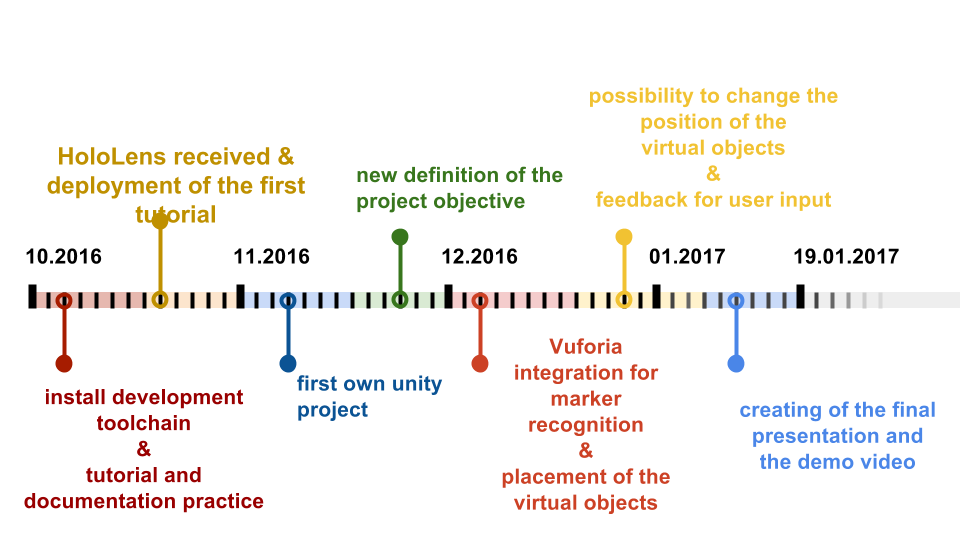
\includegraphics[width=\columnwidth]{images/Milestones.png}
	\caption{Milestones of phase I.}\label{fig:milestones}
\end{figure}

\section{Goals of Phase I}
The primary goal is to display a virtual load bar at the position of the physical load bar. In a real world scenario this should simplify the control of the stage machinery because the operator is still able to see all load bars, even if they are occluded by other objects.

In addition to that, some meta-information about the load bar is to be displayed next to said virtual load bar. For example a unique ID, the current position and the velocity are useful information for the operator that may increase the overall safety.

Furthermore it a virtual scenery shall be attached to the load bar. This corresponds with the desire for the possibility of virtual stage design as it has been described in section \ref{sec:motivation}.

\section{Roadmap}
This section contains some tentative projections on how the project might develop in the upcoming semesters/phases. 
\begin{itemize}
\item Phase I (until January 2017)
	\begin{itemize}
    \item Superimpose a virtual load bar over the physical one
    \item Display information near said virtual load bar  
    \item Attach a virtual scenery (i.e. poster) to the virtual load bar  
    \end{itemize}
\item Phase II (until June 2017)
	\begin{itemize}
    \item Receive information over the network  
    \item Position the virtual objects according to the received information   
    \end{itemize}
\item Phase III (vision)
	\begin{itemize}
    \item Multiple virtual objects/the whole stage 
    \item Integration with real stage machinery, both with a physical (miniature) stage and with stage control software
    \end{itemize}
\end{itemize}


\section{Organization}
After some experimentation with H-DA internal recourses (Perforce and Moodle) we settled on GitLab as our primary source control platform. We also use it as a document management system by adding session protocols and documentation. This is manly due to the fact that it allows for easy, self-governing repository management  and reliable, configuration free access, particularly from outside the university network. Additional features like hosting of a project website have not yet been used, but should perhaps be considered in the future, especially for documentation purposes.
